\section{Istruzione LPM}
L' istruzione LPM (Load Program Memory) permette di leggere dati dalla flash e porle all' interno di un registro.
Questo può tornare utile perché all' interno della flash poniamo i valori costanti come le stringhe, le lookup table, ecc.
Legge 1 byte per volta quindi non una riga intera!
Per indirizzare una cella si usa il registro $Z$ ma la sintassi dell' indirizzo è particolare:
\begin{figure}[H]
    \centering
    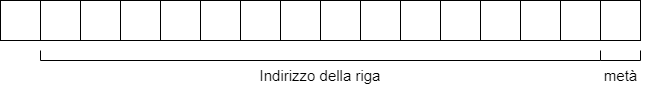
\includegraphics[width=300px]{images/8_LPM/LPM_sintassi.png}
\end{figure}
sui 16 bit del registro $Z$ i 14 bit centrali contengono l'indirizzo della riga da leggere, il bit meno significativo contiene un bit che indica:
\begin{itemize}
    \item 0: metà inferiore della riga
    \item 1: metà superiore della riga
\end{itemize}
il bit più significativo invece non è usato.

Supponiamo dunque di voler leggere alla cella con etichetta STRINGA:
\begin{verbatim}
    LDI ZL, low(STRINGA*2)
    LDI ZH, high(STRINGA*2)
    LPM
\end{verbatim}
le "funzioni" \emph{low} e \emph{high} si usano per dire all'assemblatore di prendere la parte alta o la parte bassa di un valore a 16 bit.
Inoltre l'istruzione ha un indirizzamento implicito, infatti non diamo nessun parametro, legge l'indirizzo da $Z$ e pone il byte letto in r0, in fine incrementa $Z$ di 1, in questo modo ora punterà al byte più significativo della riga.
Di fatto la sintassi di LPM è come se fosse:
\begin{verbatim}
    LPM r0, Z+
\end{verbatim}

Questo auto-incremento è utile per l'utilizzo nei loop, usati spesso per leggere stringhe dalla FLASH, a tal proposito una stringa nella FLASH si usa terminarla con un byte nullo, quindi per leggerla si potrebbe usare:
\begin{verbatim}
        LDI ZL, low(STRINGA*2)
        LDI ZH, high(STRINGA*2)
    corpo_lettura:
        LPM
        TST r0
        BREQ fuori
            ; uso del carattere in r0
        RJMP corpo_lettura
    fuori:
\end{verbatim}












